\documentclass[border=10pt]{standalone}
\usepackage{pgf,tikz,pgfplots}
\usetikzlibrary{quotes, angles}
\usetikzlibrary{positioning}
\usetikzlibrary{arrows.meta}
\usetikzlibrary{calc, shapes, automata, fit}
\tikzset{%
	% Specifications for style of nodes:
	base/.style = {rectangle, rounded corners, draw=black,
		%		minimum width=4cm, minimum height=1cm,
		inner sep=15pt,
		text centered, font=\sffamily}, 
	activityStarts/.style = {base, fill=blue!30},
	startstop/.style = {base, fill=red!30},
	activityRuns/.style = {base, fill=red!30},
	process/.style = {base, minimum width=2.5cm, fill=orange!15,
		font=\ttfamily},
	context/.style = {base, inner sep=5pt, align=justify, fill=blue!30}
}
\begin{document}
	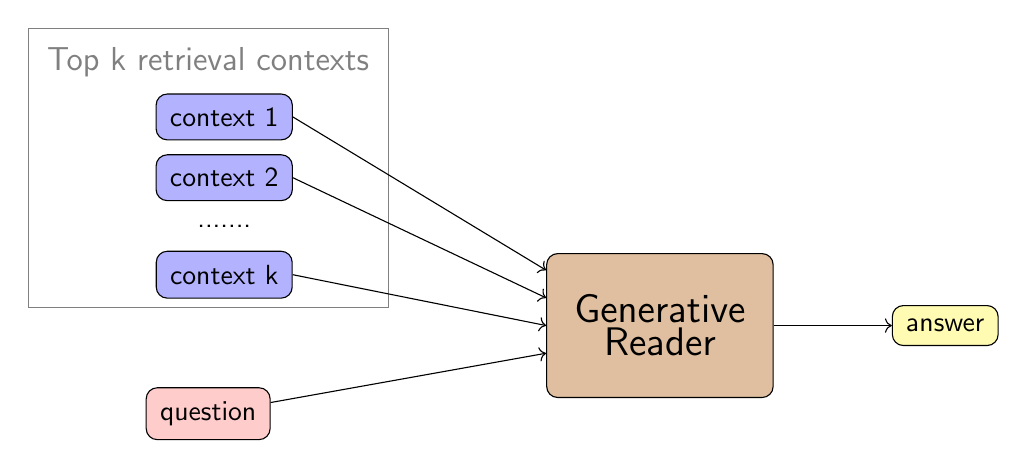
\begin{tikzpicture}[every node/.style={font=\sffamily}, align=center]
		\node (ctxs1) [context] {context 1};
		\node (ctxs2) [context, below=5pt of ctxs1] {context 2};
		\node (dots) [below=5pt of ctxs2] {.......};
		\node (ctxsk) [context, below=5pt of dots] {context k};
		\path let
		\p1 = (ctxs1.north),
		\p2 = (ctxs1.west)
		in
		coordinate (northCtxs) at (\x2, \y1);
		\node (topK) [anchor=west, shift={(-1.5cm, 0.4cm)},font=\fontsize{12pt}{\baselineskip}\selectfont\color{black!50}\sffamily] at (northCtxs) {Top k retrieval contexts};
		\node (topKblock) [draw=black!50, fit={(ctxs1) (ctxs2) (dots) (ctxsk) (topK)}] {};
		\node (question) [rounded corners, fill=red!20, draw=black, below=1cm of topKblock, inner sep=5pt] {question};
		\node (genReader) [yshift=-2cm, right=2cm of topKblock, draw=black, rounded corners, fill=brown!50, inner xsep=10pt, inner ysep=15pt, font=\fontsize{14pt}{\baselineskip}\selectfont\sffamily] {Generative \\ Reader};
		\draw[->] (ctxs1.east) -- ([yshift=20pt]genReader.west);
		\draw[->] (ctxs2.east) -- ([yshift=10pt]genReader.west);
		\draw[->] (ctxsk.east) -- (genReader.west);
		\draw[->] (question) -- ([yshift=-10pt]genReader.west);
		\node (answer) [draw=black, right=1.5cm of genReader, fill=yellow!30, rounded corners, inner sep=5pt] {answer};
		\draw[->] (genReader.east) -- (answer.west);
	\end{tikzpicture}
\end{document}